\documentclass[twoside]{book}

% Packages required by doxygen
\usepackage{fixltx2e}
\usepackage{calc}
\usepackage{doxygen}
\usepackage[export]{adjustbox} % also loads graphicx
\usepackage{graphicx}
\usepackage[utf8]{inputenc}
\usepackage{makeidx}
\usepackage{multicol}
\usepackage{multirow}
\PassOptionsToPackage{warn}{textcomp}
\usepackage{textcomp}
\usepackage[nointegrals]{wasysym}
\usepackage[table]{xcolor}

% Font selection
\usepackage[T1]{fontenc}
\usepackage[scaled=.90]{helvet}
\usepackage{courier}
\usepackage{amssymb}
\usepackage{sectsty}
\renewcommand{\familydefault}{\sfdefault}
\allsectionsfont{%
  \fontseries{bc}\selectfont%
  \color{darkgray}%
}
\renewcommand{\DoxyLabelFont}{%
  \fontseries{bc}\selectfont%
  \color{darkgray}%
}
\newcommand{\+}{\discretionary{\mbox{\scriptsize$\hookleftarrow$}}{}{}}

% Page & text layout
\usepackage{geometry}
\geometry{%
  a4paper,%
  top=2.5cm,%
  bottom=2.5cm,%
  left=2.5cm,%
  right=2.5cm%
}
\tolerance=750
\hfuzz=15pt
\hbadness=750
\setlength{\emergencystretch}{15pt}
\setlength{\parindent}{0cm}
\setlength{\parskip}{3ex plus 2ex minus 2ex}
\makeatletter
\renewcommand{\paragraph}{%
  \@startsection{paragraph}{4}{0ex}{-1.0ex}{1.0ex}{%
    \normalfont\normalsize\bfseries\SS@parafont%
  }%
}
\renewcommand{\subparagraph}{%
  \@startsection{subparagraph}{5}{0ex}{-1.0ex}{1.0ex}{%
    \normalfont\normalsize\bfseries\SS@subparafont%
  }%
}
\makeatother

% Headers & footers
\usepackage{fancyhdr}
\pagestyle{fancyplain}
\fancyhead[LE]{\fancyplain{}{\bfseries\thepage}}
\fancyhead[CE]{\fancyplain{}{}}
\fancyhead[RE]{\fancyplain{}{\bfseries\leftmark}}
\fancyhead[LO]{\fancyplain{}{\bfseries\rightmark}}
\fancyhead[CO]{\fancyplain{}{}}
\fancyhead[RO]{\fancyplain{}{\bfseries\thepage}}
\fancyfoot[LE]{\fancyplain{}{}}
\fancyfoot[CE]{\fancyplain{}{}}
\fancyfoot[RE]{\fancyplain{}{\bfseries\scriptsize Generated by Doxygen }}
\fancyfoot[LO]{\fancyplain{}{\bfseries\scriptsize Generated by Doxygen }}
\fancyfoot[CO]{\fancyplain{}{}}
\fancyfoot[RO]{\fancyplain{}{}}
\renewcommand{\footrulewidth}{0.4pt}
\renewcommand{\chaptermark}[1]{%
  \markboth{#1}{}%
}
\renewcommand{\sectionmark}[1]{%
  \markright{\thesection\ #1}%
}

% Indices & bibliography
\usepackage{natbib}
\usepackage[titles]{tocloft}
\setcounter{tocdepth}{3}
\setcounter{secnumdepth}{5}
\makeindex

% Hyperlinks (required, but should be loaded last)
\usepackage{ifpdf}
\ifpdf
  \usepackage[pdftex,pagebackref=true]{hyperref}
\else
  \usepackage[ps2pdf,pagebackref=true]{hyperref}
\fi
\hypersetup{%
  colorlinks=true,%
  linkcolor=blue,%
  citecolor=blue,%
  unicode%
}

% Custom commands
\newcommand{\clearemptydoublepage}{%
  \newpage{\pagestyle{empty}\cleardoublepage}%
}

\usepackage{caption}
\captionsetup{labelsep=space,justification=centering,font={bf},singlelinecheck=off,skip=4pt,position=top}

%===== C O N T E N T S =====

\begin{document}

% Titlepage & ToC
\hypersetup{pageanchor=false,
             bookmarksnumbered=true,
             pdfencoding=unicode
            }
\pagenumbering{alph}
\begin{titlepage}
\vspace*{7cm}
\begin{center}%
{\Large labo\+\_\+07\+\_\+schaufelberger\+\_\+yannick\+\_\+gallay\+\_\+david }\\
\vspace*{1cm}
{\large Generated by Doxygen 1.8.13}\\
\end{center}
\end{titlepage}
\clearemptydoublepage
\pagenumbering{roman}
\tableofcontents
\clearemptydoublepage
\pagenumbering{arabic}
\hypersetup{pageanchor=true}

%--- Begin generated contents ---
\chapter{File Index}
\section{File List}
Here is a list of all files with brief descriptions\+:\begin{DoxyCompactList}
\item\contentsline{section}{\hyperlink{constants_8h}{constants.\+h} }{\pageref{constants_8h}}{}
\item\contentsline{section}{\hyperlink{delta__date_8h}{delta\+\_\+date.\+h} }{\pageref{delta__date_8h}}{}
\item\contentsline{section}{\hyperlink{interface_8h}{interface.\+h} }{\pageref{interface_8h}}{}
\item\contentsline{section}{\hyperlink{utilities_8h}{utilities.\+h} }{\pageref{utilities_8h}}{}
\end{DoxyCompactList}

\chapter{File Documentation}
\hypertarget{constants_8h}{}\section{constants.\+h File Reference}
\label{constants_8h}\index{constants.\+h@{constants.\+h}}
\subsection*{Enumerations}
\begin{DoxyCompactItemize}
\item 
enum \hyperlink{constants_8h_a5319f32c533a734bb70a5da75a91b489}{M\+O\+N\+T\+HS} \{ \newline
\hyperlink{constants_8h_a5319f32c533a734bb70a5da75a91b489a9b99b7174c17b3d40f9a2e05b794b150}{J\+A\+N\+U\+AR} = 1, 
\hyperlink{constants_8h_a5319f32c533a734bb70a5da75a91b489a78d9292c615262d4def8fcd5b36ebcde}{F\+E\+B\+R\+U\+AR}, 
\hyperlink{constants_8h_a5319f32c533a734bb70a5da75a91b489a9643d50b680531fd28efd57d52e86d41}{M\+A\+R\+CH}, 
\hyperlink{constants_8h_a5319f32c533a734bb70a5da75a91b489aecd9e52062ac25b7b4653ce5553531c6}{A\+P\+R\+IL}, 
\newline
\hyperlink{constants_8h_a5319f32c533a734bb70a5da75a91b489ab6c4cee5488c943c81d62122822830e4}{M\+AY}, 
\hyperlink{constants_8h_a5319f32c533a734bb70a5da75a91b489a945a352d55e34c81e027654c0209f509}{J\+U\+NE}, 
\hyperlink{constants_8h_a5319f32c533a734bb70a5da75a91b489ad645b2396112d5d9a33ec2acc0d23519}{J\+U\+LY}, 
\hyperlink{constants_8h_a5319f32c533a734bb70a5da75a91b489ab40cf84788c0a5a41375e30063586b7f}{A\+U\+G\+U\+ST}, 
\newline
\hyperlink{constants_8h_a5319f32c533a734bb70a5da75a91b489ad3da1ebcdb93dbc04b8cd63b7e1bc84b}{S\+E\+P\+T\+E\+M\+B\+ER}, 
\hyperlink{constants_8h_a5319f32c533a734bb70a5da75a91b489a554aba97586ee43f0ca51b0089eed03c}{O\+C\+T\+O\+B\+ER}, 
\hyperlink{constants_8h_a5319f32c533a734bb70a5da75a91b489a3356ccc34e34421d48e6c4b1e68515fe}{N\+O\+V\+E\+M\+B\+ER}, 
\hyperlink{constants_8h_a5319f32c533a734bb70a5da75a91b489a823acaf8f57efe16924d4233a9547c03}{D\+E\+C\+E\+M\+B\+ER}
 \}
\end{DoxyCompactItemize}
\subsection*{Variables}
\begin{DoxyCompactItemize}
\item 
const int \hyperlink{constants_8h_a4907347b8683a20563d85aa2441486d9}{M\+I\+N\+\_\+\+D\+AY} = 1
\item 
const int \hyperlink{constants_8h_a1919ac299561571f7be9706d922c000f}{M\+I\+N\+\_\+\+M\+O\+N\+TH} = \hyperlink{constants_8h_a5319f32c533a734bb70a5da75a91b489a9b99b7174c17b3d40f9a2e05b794b150}{J\+A\+N\+U\+AR}
\item 
const int \hyperlink{constants_8h_aaa38a368ef23591e9f77be2ae3ff414e}{M\+I\+N\+\_\+\+Y\+E\+AR} = 1900
\item 
const int \hyperlink{constants_8h_a11efe6da26a907e42ed60692a4653ee3}{M\+A\+X\+\_\+\+D\+AY} = 31
\item 
const int \hyperlink{constants_8h_af40377af64048f01ccb27201536c2409}{M\+A\+X\+\_\+\+M\+O\+N\+TH} = \hyperlink{constants_8h_a5319f32c533a734bb70a5da75a91b489a823acaf8f57efe16924d4233a9547c03}{D\+E\+C\+E\+M\+B\+ER}
\item 
const int \hyperlink{constants_8h_a6e0f9f2f5acbac3eeb73fc6e2f0d0053}{M\+A\+X\+\_\+\+Y\+E\+AR} = 2300
\item 
const char \hyperlink{constants_8h_a7d2919284d7da447f920c583412e69d8}{D\+A\+T\+E\+\_\+\+S\+E\+P\+A\+R\+A\+T\+OR} = \textquotesingle{}-\/\textquotesingle{}
\end{DoxyCompactItemize}


\subsection{Enumeration Type Documentation}
\mbox{\Hypertarget{constants_8h_a5319f32c533a734bb70a5da75a91b489}\label{constants_8h_a5319f32c533a734bb70a5da75a91b489}} 
\index{constants.\+h@{constants.\+h}!M\+O\+N\+T\+HS@{M\+O\+N\+T\+HS}}
\index{M\+O\+N\+T\+HS@{M\+O\+N\+T\+HS}!constants.\+h@{constants.\+h}}
\subsubsection{\texorpdfstring{M\+O\+N\+T\+HS}{MONTHS}}
{\footnotesize\ttfamily enum \hyperlink{constants_8h_a5319f32c533a734bb70a5da75a91b489}{M\+O\+N\+T\+HS}}

\begin{DoxyEnumFields}{Enumerator}
\raisebox{\heightof{T}}[0pt][0pt]{\index{J\+A\+N\+U\+AR@{J\+A\+N\+U\+AR}!constants.\+h@{constants.\+h}}\index{constants.\+h@{constants.\+h}!J\+A\+N\+U\+AR@{J\+A\+N\+U\+AR}}}\mbox{\Hypertarget{constants_8h_a5319f32c533a734bb70a5da75a91b489a9b99b7174c17b3d40f9a2e05b794b150}\label{constants_8h_a5319f32c533a734bb70a5da75a91b489a9b99b7174c17b3d40f9a2e05b794b150}} 
J\+A\+N\+U\+AR&\\
\hline

\raisebox{\heightof{T}}[0pt][0pt]{\index{F\+E\+B\+R\+U\+AR@{F\+E\+B\+R\+U\+AR}!constants.\+h@{constants.\+h}}\index{constants.\+h@{constants.\+h}!F\+E\+B\+R\+U\+AR@{F\+E\+B\+R\+U\+AR}}}\mbox{\Hypertarget{constants_8h_a5319f32c533a734bb70a5da75a91b489a78d9292c615262d4def8fcd5b36ebcde}\label{constants_8h_a5319f32c533a734bb70a5da75a91b489a78d9292c615262d4def8fcd5b36ebcde}} 
F\+E\+B\+R\+U\+AR&\\
\hline

\raisebox{\heightof{T}}[0pt][0pt]{\index{M\+A\+R\+CH@{M\+A\+R\+CH}!constants.\+h@{constants.\+h}}\index{constants.\+h@{constants.\+h}!M\+A\+R\+CH@{M\+A\+R\+CH}}}\mbox{\Hypertarget{constants_8h_a5319f32c533a734bb70a5da75a91b489a9643d50b680531fd28efd57d52e86d41}\label{constants_8h_a5319f32c533a734bb70a5da75a91b489a9643d50b680531fd28efd57d52e86d41}} 
M\+A\+R\+CH&\\
\hline

\raisebox{\heightof{T}}[0pt][0pt]{\index{A\+P\+R\+IL@{A\+P\+R\+IL}!constants.\+h@{constants.\+h}}\index{constants.\+h@{constants.\+h}!A\+P\+R\+IL@{A\+P\+R\+IL}}}\mbox{\Hypertarget{constants_8h_a5319f32c533a734bb70a5da75a91b489aecd9e52062ac25b7b4653ce5553531c6}\label{constants_8h_a5319f32c533a734bb70a5da75a91b489aecd9e52062ac25b7b4653ce5553531c6}} 
A\+P\+R\+IL&\\
\hline

\raisebox{\heightof{T}}[0pt][0pt]{\index{M\+AY@{M\+AY}!constants.\+h@{constants.\+h}}\index{constants.\+h@{constants.\+h}!M\+AY@{M\+AY}}}\mbox{\Hypertarget{constants_8h_a5319f32c533a734bb70a5da75a91b489ab6c4cee5488c943c81d62122822830e4}\label{constants_8h_a5319f32c533a734bb70a5da75a91b489ab6c4cee5488c943c81d62122822830e4}} 
M\+AY&\\
\hline

\raisebox{\heightof{T}}[0pt][0pt]{\index{J\+U\+NE@{J\+U\+NE}!constants.\+h@{constants.\+h}}\index{constants.\+h@{constants.\+h}!J\+U\+NE@{J\+U\+NE}}}\mbox{\Hypertarget{constants_8h_a5319f32c533a734bb70a5da75a91b489a945a352d55e34c81e027654c0209f509}\label{constants_8h_a5319f32c533a734bb70a5da75a91b489a945a352d55e34c81e027654c0209f509}} 
J\+U\+NE&\\
\hline

\raisebox{\heightof{T}}[0pt][0pt]{\index{J\+U\+LY@{J\+U\+LY}!constants.\+h@{constants.\+h}}\index{constants.\+h@{constants.\+h}!J\+U\+LY@{J\+U\+LY}}}\mbox{\Hypertarget{constants_8h_a5319f32c533a734bb70a5da75a91b489ad645b2396112d5d9a33ec2acc0d23519}\label{constants_8h_a5319f32c533a734bb70a5da75a91b489ad645b2396112d5d9a33ec2acc0d23519}} 
J\+U\+LY&\\
\hline

\raisebox{\heightof{T}}[0pt][0pt]{\index{A\+U\+G\+U\+ST@{A\+U\+G\+U\+ST}!constants.\+h@{constants.\+h}}\index{constants.\+h@{constants.\+h}!A\+U\+G\+U\+ST@{A\+U\+G\+U\+ST}}}\mbox{\Hypertarget{constants_8h_a5319f32c533a734bb70a5da75a91b489ab40cf84788c0a5a41375e30063586b7f}\label{constants_8h_a5319f32c533a734bb70a5da75a91b489ab40cf84788c0a5a41375e30063586b7f}} 
A\+U\+G\+U\+ST&\\
\hline

\raisebox{\heightof{T}}[0pt][0pt]{\index{S\+E\+P\+T\+E\+M\+B\+ER@{S\+E\+P\+T\+E\+M\+B\+ER}!constants.\+h@{constants.\+h}}\index{constants.\+h@{constants.\+h}!S\+E\+P\+T\+E\+M\+B\+ER@{S\+E\+P\+T\+E\+M\+B\+ER}}}\mbox{\Hypertarget{constants_8h_a5319f32c533a734bb70a5da75a91b489ad3da1ebcdb93dbc04b8cd63b7e1bc84b}\label{constants_8h_a5319f32c533a734bb70a5da75a91b489ad3da1ebcdb93dbc04b8cd63b7e1bc84b}} 
S\+E\+P\+T\+E\+M\+B\+ER&\\
\hline

\raisebox{\heightof{T}}[0pt][0pt]{\index{O\+C\+T\+O\+B\+ER@{O\+C\+T\+O\+B\+ER}!constants.\+h@{constants.\+h}}\index{constants.\+h@{constants.\+h}!O\+C\+T\+O\+B\+ER@{O\+C\+T\+O\+B\+ER}}}\mbox{\Hypertarget{constants_8h_a5319f32c533a734bb70a5da75a91b489a554aba97586ee43f0ca51b0089eed03c}\label{constants_8h_a5319f32c533a734bb70a5da75a91b489a554aba97586ee43f0ca51b0089eed03c}} 
O\+C\+T\+O\+B\+ER&\\
\hline

\raisebox{\heightof{T}}[0pt][0pt]{\index{N\+O\+V\+E\+M\+B\+ER@{N\+O\+V\+E\+M\+B\+ER}!constants.\+h@{constants.\+h}}\index{constants.\+h@{constants.\+h}!N\+O\+V\+E\+M\+B\+ER@{N\+O\+V\+E\+M\+B\+ER}}}\mbox{\Hypertarget{constants_8h_a5319f32c533a734bb70a5da75a91b489a3356ccc34e34421d48e6c4b1e68515fe}\label{constants_8h_a5319f32c533a734bb70a5da75a91b489a3356ccc34e34421d48e6c4b1e68515fe}} 
N\+O\+V\+E\+M\+B\+ER&\\
\hline

\raisebox{\heightof{T}}[0pt][0pt]{\index{D\+E\+C\+E\+M\+B\+ER@{D\+E\+C\+E\+M\+B\+ER}!constants.\+h@{constants.\+h}}\index{constants.\+h@{constants.\+h}!D\+E\+C\+E\+M\+B\+ER@{D\+E\+C\+E\+M\+B\+ER}}}\mbox{\Hypertarget{constants_8h_a5319f32c533a734bb70a5da75a91b489a823acaf8f57efe16924d4233a9547c03}\label{constants_8h_a5319f32c533a734bb70a5da75a91b489a823acaf8f57efe16924d4233a9547c03}} 
D\+E\+C\+E\+M\+B\+ER&\\
\hline

\end{DoxyEnumFields}


\subsection{Variable Documentation}
\mbox{\Hypertarget{constants_8h_a7d2919284d7da447f920c583412e69d8}\label{constants_8h_a7d2919284d7da447f920c583412e69d8}} 
\index{constants.\+h@{constants.\+h}!D\+A\+T\+E\+\_\+\+S\+E\+P\+A\+R\+A\+T\+OR@{D\+A\+T\+E\+\_\+\+S\+E\+P\+A\+R\+A\+T\+OR}}
\index{D\+A\+T\+E\+\_\+\+S\+E\+P\+A\+R\+A\+T\+OR@{D\+A\+T\+E\+\_\+\+S\+E\+P\+A\+R\+A\+T\+OR}!constants.\+h@{constants.\+h}}
\subsubsection{\texorpdfstring{D\+A\+T\+E\+\_\+\+S\+E\+P\+A\+R\+A\+T\+OR}{DATE\_SEPARATOR}}
{\footnotesize\ttfamily const char D\+A\+T\+E\+\_\+\+S\+E\+P\+A\+R\+A\+T\+OR = \textquotesingle{}-\/\textquotesingle{}}

\mbox{\Hypertarget{constants_8h_a11efe6da26a907e42ed60692a4653ee3}\label{constants_8h_a11efe6da26a907e42ed60692a4653ee3}} 
\index{constants.\+h@{constants.\+h}!M\+A\+X\+\_\+\+D\+AY@{M\+A\+X\+\_\+\+D\+AY}}
\index{M\+A\+X\+\_\+\+D\+AY@{M\+A\+X\+\_\+\+D\+AY}!constants.\+h@{constants.\+h}}
\subsubsection{\texorpdfstring{M\+A\+X\+\_\+\+D\+AY}{MAX\_DAY}}
{\footnotesize\ttfamily const int M\+A\+X\+\_\+\+D\+AY = 31}

\mbox{\Hypertarget{constants_8h_af40377af64048f01ccb27201536c2409}\label{constants_8h_af40377af64048f01ccb27201536c2409}} 
\index{constants.\+h@{constants.\+h}!M\+A\+X\+\_\+\+M\+O\+N\+TH@{M\+A\+X\+\_\+\+M\+O\+N\+TH}}
\index{M\+A\+X\+\_\+\+M\+O\+N\+TH@{M\+A\+X\+\_\+\+M\+O\+N\+TH}!constants.\+h@{constants.\+h}}
\subsubsection{\texorpdfstring{M\+A\+X\+\_\+\+M\+O\+N\+TH}{MAX\_MONTH}}
{\footnotesize\ttfamily const int M\+A\+X\+\_\+\+M\+O\+N\+TH = \hyperlink{constants_8h_a5319f32c533a734bb70a5da75a91b489a823acaf8f57efe16924d4233a9547c03}{D\+E\+C\+E\+M\+B\+ER}}

\mbox{\Hypertarget{constants_8h_a6e0f9f2f5acbac3eeb73fc6e2f0d0053}\label{constants_8h_a6e0f9f2f5acbac3eeb73fc6e2f0d0053}} 
\index{constants.\+h@{constants.\+h}!M\+A\+X\+\_\+\+Y\+E\+AR@{M\+A\+X\+\_\+\+Y\+E\+AR}}
\index{M\+A\+X\+\_\+\+Y\+E\+AR@{M\+A\+X\+\_\+\+Y\+E\+AR}!constants.\+h@{constants.\+h}}
\subsubsection{\texorpdfstring{M\+A\+X\+\_\+\+Y\+E\+AR}{MAX\_YEAR}}
{\footnotesize\ttfamily const int M\+A\+X\+\_\+\+Y\+E\+AR = 2300}

\mbox{\Hypertarget{constants_8h_a4907347b8683a20563d85aa2441486d9}\label{constants_8h_a4907347b8683a20563d85aa2441486d9}} 
\index{constants.\+h@{constants.\+h}!M\+I\+N\+\_\+\+D\+AY@{M\+I\+N\+\_\+\+D\+AY}}
\index{M\+I\+N\+\_\+\+D\+AY@{M\+I\+N\+\_\+\+D\+AY}!constants.\+h@{constants.\+h}}
\subsubsection{\texorpdfstring{M\+I\+N\+\_\+\+D\+AY}{MIN\_DAY}}
{\footnotesize\ttfamily const int M\+I\+N\+\_\+\+D\+AY = 1}

\mbox{\Hypertarget{constants_8h_a1919ac299561571f7be9706d922c000f}\label{constants_8h_a1919ac299561571f7be9706d922c000f}} 
\index{constants.\+h@{constants.\+h}!M\+I\+N\+\_\+\+M\+O\+N\+TH@{M\+I\+N\+\_\+\+M\+O\+N\+TH}}
\index{M\+I\+N\+\_\+\+M\+O\+N\+TH@{M\+I\+N\+\_\+\+M\+O\+N\+TH}!constants.\+h@{constants.\+h}}
\subsubsection{\texorpdfstring{M\+I\+N\+\_\+\+M\+O\+N\+TH}{MIN\_MONTH}}
{\footnotesize\ttfamily const int M\+I\+N\+\_\+\+M\+O\+N\+TH = \hyperlink{constants_8h_a5319f32c533a734bb70a5da75a91b489a9b99b7174c17b3d40f9a2e05b794b150}{J\+A\+N\+U\+AR}}

\mbox{\Hypertarget{constants_8h_aaa38a368ef23591e9f77be2ae3ff414e}\label{constants_8h_aaa38a368ef23591e9f77be2ae3ff414e}} 
\index{constants.\+h@{constants.\+h}!M\+I\+N\+\_\+\+Y\+E\+AR@{M\+I\+N\+\_\+\+Y\+E\+AR}}
\index{M\+I\+N\+\_\+\+Y\+E\+AR@{M\+I\+N\+\_\+\+Y\+E\+AR}!constants.\+h@{constants.\+h}}
\subsubsection{\texorpdfstring{M\+I\+N\+\_\+\+Y\+E\+AR}{MIN\_YEAR}}
{\footnotesize\ttfamily const int M\+I\+N\+\_\+\+Y\+E\+AR = 1900}


\hypertarget{delta__date_8h}{}\section{delta\+\_\+date.\+h File Reference}
\label{delta__date_8h}\index{delta\+\_\+date.\+h@{delta\+\_\+date.\+h}}
{\ttfamily \#include $<$string$>$}\newline
Include dependency graph for delta\+\_\+date.\+h\+:
\nopagebreak
\begin{figure}[H]
\begin{center}
\leavevmode
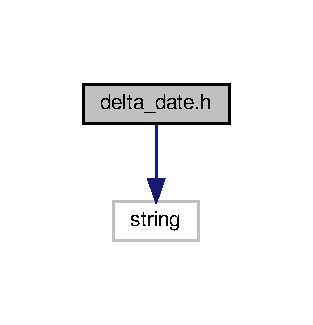
\includegraphics[width=150pt]{delta__date_8h__incl}
\end{center}
\end{figure}
\subsection*{Functions}
\begin{DoxyCompactItemize}
\item 
bool \hyperlink{delta__date_8h_a74d9e16c629fb46c9f168d924536e53c}{ignore\+\_\+date\+\_\+separator} ()
\begin{DoxyCompactList}\small\item\em This function clears the next character in the buffer, and returns true if it isn\textquotesingle{}t D\+A\+T\+E\+\_\+\+S\+E\+P\+A\+R\+A\+T\+OR. \end{DoxyCompactList}\item 
bool \hyperlink{delta__date_8h_abb8c4657bfbda629fd7ce0435d354637}{ask\+\_\+date} (const std\+::string \&date, int \&day, int \&month, int \&year)
\begin{DoxyCompactList}\small\item\em This function modifies the three referenced arguments to values inputted by the user. \end{DoxyCompactList}\item 
void \hyperlink{delta__date_8h_a661ee7feb8e24a8f63ea228865031ae8}{ask\+\_\+for\+\_\+valid\+\_\+date} (const std\+::string \&date, int \&day, int \&month, int \&year)
\begin{DoxyCompactList}\small\item\em This function asks for a valid date with the format D\+D-\/\+M\+M-\/\+Y\+Y\+YY using ask\+\_\+date function. As long as the date is invalid, or the format is wrong, it asks for a new date. \end{DoxyCompactList}\item 
void \hyperlink{delta__date_8h_a0aa00c0e9c3ebb2aaf65a7ccfffb6e86}{ask\+\_\+and\+\_\+compute\+\_\+delta\+\_\+day\+\_\+between\+\_\+two\+\_\+dates} ()
\begin{DoxyCompactList}\small\item\em This function asks for a valid dates within a given range of dates in format D\+D-\/\+M\+M-\/\+Y\+Y\+YY and display the number of day between the choosen dates. \end{DoxyCompactList}\end{DoxyCompactItemize}


\subsection{Function Documentation}
\mbox{\Hypertarget{delta__date_8h_a0aa00c0e9c3ebb2aaf65a7ccfffb6e86}\label{delta__date_8h_a0aa00c0e9c3ebb2aaf65a7ccfffb6e86}} 
\index{delta\+\_\+date.\+h@{delta\+\_\+date.\+h}!ask\+\_\+and\+\_\+compute\+\_\+delta\+\_\+day\+\_\+between\+\_\+two\+\_\+dates@{ask\+\_\+and\+\_\+compute\+\_\+delta\+\_\+day\+\_\+between\+\_\+two\+\_\+dates}}
\index{ask\+\_\+and\+\_\+compute\+\_\+delta\+\_\+day\+\_\+between\+\_\+two\+\_\+dates@{ask\+\_\+and\+\_\+compute\+\_\+delta\+\_\+day\+\_\+between\+\_\+two\+\_\+dates}!delta\+\_\+date.\+h@{delta\+\_\+date.\+h}}
\subsubsection{\texorpdfstring{ask\+\_\+and\+\_\+compute\+\_\+delta\+\_\+day\+\_\+between\+\_\+two\+\_\+dates()}{ask\_and\_compute\_delta\_day\_between\_two\_dates()}}
{\footnotesize\ttfamily void ask\+\_\+and\+\_\+compute\+\_\+delta\+\_\+day\+\_\+between\+\_\+two\+\_\+dates (\begin{DoxyParamCaption}{ }\end{DoxyParamCaption})}



This function asks for a valid dates within a given range of dates in format D\+D-\/\+M\+M-\/\+Y\+Y\+YY and display the number of day between the choosen dates. 

\mbox{\Hypertarget{delta__date_8h_abb8c4657bfbda629fd7ce0435d354637}\label{delta__date_8h_abb8c4657bfbda629fd7ce0435d354637}} 
\index{delta\+\_\+date.\+h@{delta\+\_\+date.\+h}!ask\+\_\+date@{ask\+\_\+date}}
\index{ask\+\_\+date@{ask\+\_\+date}!delta\+\_\+date.\+h@{delta\+\_\+date.\+h}}
\subsubsection{\texorpdfstring{ask\+\_\+date()}{ask\_date()}}
{\footnotesize\ttfamily bool ask\+\_\+date (\begin{DoxyParamCaption}\item[{const std\+::string \&}]{date,  }\item[{int \&}]{day,  }\item[{int \&}]{month,  }\item[{int \&}]{year }\end{DoxyParamCaption})}



This function modifies the three referenced arguments to values inputted by the user. 


\begin{DoxyParams}{Parameters}
{\em date} & string telling the user if it\textquotesingle{}s the start date or end date \\
\hline
{\em day} & input of the user \\
\hline
{\em month} & input of the user \\
\hline
{\em year} & input of the user \\
\hline
\end{DoxyParams}
\begin{DoxyReturn}{Returns}
true if the date has been retrieve successfully according to D\+D-\/\+M\+M-\/\+Y\+Y\+YY format, else false 
\end{DoxyReturn}
\mbox{\Hypertarget{delta__date_8h_a661ee7feb8e24a8f63ea228865031ae8}\label{delta__date_8h_a661ee7feb8e24a8f63ea228865031ae8}} 
\index{delta\+\_\+date.\+h@{delta\+\_\+date.\+h}!ask\+\_\+for\+\_\+valid\+\_\+date@{ask\+\_\+for\+\_\+valid\+\_\+date}}
\index{ask\+\_\+for\+\_\+valid\+\_\+date@{ask\+\_\+for\+\_\+valid\+\_\+date}!delta\+\_\+date.\+h@{delta\+\_\+date.\+h}}
\subsubsection{\texorpdfstring{ask\+\_\+for\+\_\+valid\+\_\+date()}{ask\_for\_valid\_date()}}
{\footnotesize\ttfamily void ask\+\_\+for\+\_\+valid\+\_\+date (\begin{DoxyParamCaption}\item[{const std\+::string \&}]{date,  }\item[{int \&}]{day,  }\item[{int \&}]{month,  }\item[{int \&}]{year }\end{DoxyParamCaption})}



This function asks for a valid date with the format D\+D-\/\+M\+M-\/\+Y\+Y\+YY using ask\+\_\+date function. As long as the date is invalid, or the format is wrong, it asks for a new date. 


\begin{DoxyParams}{Parameters}
{\em date} & \\
\hline
{\em day} & input of the user in function \hyperlink{delta__date_8h_abb8c4657bfbda629fd7ce0435d354637}{ask\+\_\+date()} \\
\hline
{\em month} & input of the user in function \hyperlink{delta__date_8h_abb8c4657bfbda629fd7ce0435d354637}{ask\+\_\+date()} \\
\hline
{\em year} & input of the user in function \hyperlink{delta__date_8h_abb8c4657bfbda629fd7ce0435d354637}{ask\+\_\+date()} \\
\hline
\end{DoxyParams}
\mbox{\Hypertarget{delta__date_8h_a74d9e16c629fb46c9f168d924536e53c}\label{delta__date_8h_a74d9e16c629fb46c9f168d924536e53c}} 
\index{delta\+\_\+date.\+h@{delta\+\_\+date.\+h}!ignore\+\_\+date\+\_\+separator@{ignore\+\_\+date\+\_\+separator}}
\index{ignore\+\_\+date\+\_\+separator@{ignore\+\_\+date\+\_\+separator}!delta\+\_\+date.\+h@{delta\+\_\+date.\+h}}
\subsubsection{\texorpdfstring{ignore\+\_\+date\+\_\+separator()}{ignore\_date\_separator()}}
{\footnotesize\ttfamily bool ignore\+\_\+date\+\_\+separator (\begin{DoxyParamCaption}{ }\end{DoxyParamCaption})}



This function clears the next character in the buffer, and returns true if it isn\textquotesingle{}t D\+A\+T\+E\+\_\+\+S\+E\+P\+A\+R\+A\+T\+OR. 

\begin{DoxyReturn}{Returns}
false if the buffer contains the char D\+A\+T\+E\+\_\+\+S\+E\+P\+A\+R\+A\+T\+OR, true if it doesn\textquotesingle{}t 
\end{DoxyReturn}

\hypertarget{interface_8h}{}\section{interface.\+h File Reference}
\label{interface_8h}\index{interface.\+h@{interface.\+h}}
\subsection*{Functions}
\begin{DoxyCompactItemize}
\item 
bool \hyperlink{interface_8h_aa168270f51adeba28887f16bd8bb6dbb}{ask\+\_\+for\+\_\+restart} ()
\begin{DoxyCompactList}\small\item\em This function keeps asking as long as the user enters anything else than R\+E\+S\+T\+A\+R\+T\+\_\+\+C\+H\+AR or S\+T\+O\+P\+\_\+\+C\+H\+AR. \end{DoxyCompactList}\end{DoxyCompactItemize}
\subsection*{Variables}
\begin{DoxyCompactItemize}
\item 
const char \hyperlink{interface_8h_a9efb394418d13b602a0cd1c9a62e9e98}{R\+E\+S\+T\+A\+R\+T\+\_\+\+C\+H\+AR} = \textquotesingle{}O\textquotesingle{}
\item 
const char \hyperlink{interface_8h_a1b0f30495c3ac4d4dd8e09c8b3b8c506}{S\+T\+O\+P\+\_\+\+C\+H\+AR} = \textquotesingle{}N\textquotesingle{}
\end{DoxyCompactItemize}


\subsection{Function Documentation}
\mbox{\Hypertarget{interface_8h_aa168270f51adeba28887f16bd8bb6dbb}\label{interface_8h_aa168270f51adeba28887f16bd8bb6dbb}} 
\index{interface.\+h@{interface.\+h}!ask\+\_\+for\+\_\+restart@{ask\+\_\+for\+\_\+restart}}
\index{ask\+\_\+for\+\_\+restart@{ask\+\_\+for\+\_\+restart}!interface.\+h@{interface.\+h}}
\subsubsection{\texorpdfstring{ask\+\_\+for\+\_\+restart()}{ask\_for\_restart()}}
{\footnotesize\ttfamily bool ask\+\_\+for\+\_\+restart (\begin{DoxyParamCaption}{ }\end{DoxyParamCaption})}



This function keeps asking as long as the user enters anything else than R\+E\+S\+T\+A\+R\+T\+\_\+\+C\+H\+AR or S\+T\+O\+P\+\_\+\+C\+H\+AR. 

\begin{DoxyReturn}{Returns}
true if the user has entered R\+E\+S\+T\+A\+R\+T\+\_\+\+C\+H\+AR and false if the user has entered S\+T\+O\+P\+\_\+\+C\+H\+AR 
\end{DoxyReturn}


\subsection{Variable Documentation}
\mbox{\Hypertarget{interface_8h_a9efb394418d13b602a0cd1c9a62e9e98}\label{interface_8h_a9efb394418d13b602a0cd1c9a62e9e98}} 
\index{interface.\+h@{interface.\+h}!R\+E\+S\+T\+A\+R\+T\+\_\+\+C\+H\+AR@{R\+E\+S\+T\+A\+R\+T\+\_\+\+C\+H\+AR}}
\index{R\+E\+S\+T\+A\+R\+T\+\_\+\+C\+H\+AR@{R\+E\+S\+T\+A\+R\+T\+\_\+\+C\+H\+AR}!interface.\+h@{interface.\+h}}
\subsubsection{\texorpdfstring{R\+E\+S\+T\+A\+R\+T\+\_\+\+C\+H\+AR}{RESTART\_CHAR}}
{\footnotesize\ttfamily const char R\+E\+S\+T\+A\+R\+T\+\_\+\+C\+H\+AR = \textquotesingle{}O\textquotesingle{}}

\mbox{\Hypertarget{interface_8h_a1b0f30495c3ac4d4dd8e09c8b3b8c506}\label{interface_8h_a1b0f30495c3ac4d4dd8e09c8b3b8c506}} 
\index{interface.\+h@{interface.\+h}!S\+T\+O\+P\+\_\+\+C\+H\+AR@{S\+T\+O\+P\+\_\+\+C\+H\+AR}}
\index{S\+T\+O\+P\+\_\+\+C\+H\+AR@{S\+T\+O\+P\+\_\+\+C\+H\+AR}!interface.\+h@{interface.\+h}}
\subsubsection{\texorpdfstring{S\+T\+O\+P\+\_\+\+C\+H\+AR}{STOP\_CHAR}}
{\footnotesize\ttfamily const char S\+T\+O\+P\+\_\+\+C\+H\+AR = \textquotesingle{}N\textquotesingle{}}


\hypertarget{utilities_8h}{}\section{utilities.\+h File Reference}
\label{utilities_8h}\index{utilities.\+h@{utilities.\+h}}
{\ttfamily \#include $<$string$>$}\newline
{\ttfamily \#include $<$iostream$>$}\newline
{\ttfamily \#include $<$limits$>$}\newline
Include dependency graph for utilities.\+h\+:
\nopagebreak
\begin{figure}[H]
\begin{center}
\leavevmode
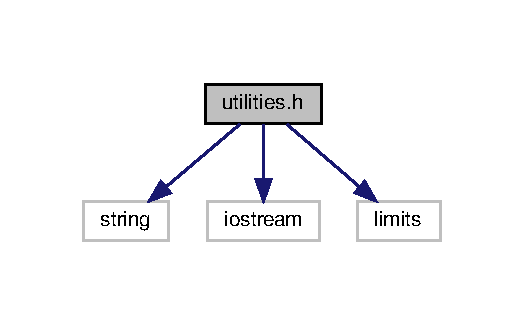
\includegraphics[width=252pt]{utilities_8h__incl}
\end{center}
\end{figure}
\subsection*{Macros}
\begin{DoxyCompactItemize}
\item 
\#define \hyperlink{utilities_8h_aa28dd17f6f34a0944a90f741b0251239}{C\+L\+E\+A\+R\+\_\+\+B\+U\+F\+F\+ER}~std\+::cin.\+ignore(std\+::numeric\+\_\+limits$<$std\+::streamsize$>$\+::max(),\textquotesingle{}\textbackslash{}n\textquotesingle{})
\end{DoxyCompactItemize}
\subsection*{Functions}
\begin{DoxyCompactItemize}
\item 
bool \hyperlink{utilities_8h_ab345f7b66a3e361e0a77d7b7cbf235b9}{is\+\_\+leap\+\_\+year} (int year)
\item 
bool \hyperlink{utilities_8h_ab4f39d1c0d3eb7f860d0c5b45cea1508}{is\+\_\+date\+\_\+valid} (int day, int month, int year)
\begin{DoxyCompactList}\small\item\em This function checks that year is between a range of date given by constants, that month is between 1 and 12 and that day is between 1 and 28/29/30/31, depending on the month. \end{DoxyCompactList}\item 
bool \hyperlink{utilities_8h_a790d01d0aefca81c0b0d0a2087164540}{check\+\_\+date\+\_\+order} (int start\+\_\+day, int start\+\_\+month, int start\+\_\+year, int end\+\_\+day, int end\+\_\+month, int end\+\_\+year)
\item 
int \hyperlink{utilities_8h_aed6999618bc3a75dc5feea6dd9a3b44c}{days\+\_\+between\+\_\+dates} (int start\+Day, int start\+Month, int start\+Year, int end\+Day, int end\+Month, int end\+Year)
\begin{DoxyCompactList}\small\item\em This returns a negative number if the start date is after the end date. \end{DoxyCompactList}\item 
int \hyperlink{utilities_8h_aa87e64a9bf33e0f48d84ce37f2020ad6}{get\+\_\+days\+\_\+since\+\_\+reference\+\_\+day} (int day, int month, int year)
\begin{DoxyCompactList}\small\item\em This function is heavily inspired by the Julian Day calculation found on this page \+: \href{http://www.cs.utsa.edu/~cs1063/projects/Spring2011/Project1/jdn-explanation.html}{\tt http\+://www.\+cs.\+utsa.\+edu/$\sim$cs1063/projects/\+Spring2011/\+Project1/jdn-\/explanation.\+html} It has been slightly modified to fit the current project. \end{DoxyCompactList}\end{DoxyCompactItemize}


\subsection{Macro Definition Documentation}
\mbox{\Hypertarget{utilities_8h_aa28dd17f6f34a0944a90f741b0251239}\label{utilities_8h_aa28dd17f6f34a0944a90f741b0251239}} 
\index{utilities.\+h@{utilities.\+h}!C\+L\+E\+A\+R\+\_\+\+B\+U\+F\+F\+ER@{C\+L\+E\+A\+R\+\_\+\+B\+U\+F\+F\+ER}}
\index{C\+L\+E\+A\+R\+\_\+\+B\+U\+F\+F\+ER@{C\+L\+E\+A\+R\+\_\+\+B\+U\+F\+F\+ER}!utilities.\+h@{utilities.\+h}}
\subsubsection{\texorpdfstring{C\+L\+E\+A\+R\+\_\+\+B\+U\+F\+F\+ER}{CLEAR\_BUFFER}}
{\footnotesize\ttfamily \#define C\+L\+E\+A\+R\+\_\+\+B\+U\+F\+F\+ER~std\+::cin.\+ignore(std\+::numeric\+\_\+limits$<$std\+::streamsize$>$\+::max(),\textquotesingle{}\textbackslash{}n\textquotesingle{})}



\subsection{Function Documentation}
\mbox{\Hypertarget{utilities_8h_a790d01d0aefca81c0b0d0a2087164540}\label{utilities_8h_a790d01d0aefca81c0b0d0a2087164540}} 
\index{utilities.\+h@{utilities.\+h}!check\+\_\+date\+\_\+order@{check\+\_\+date\+\_\+order}}
\index{check\+\_\+date\+\_\+order@{check\+\_\+date\+\_\+order}!utilities.\+h@{utilities.\+h}}
\subsubsection{\texorpdfstring{check\+\_\+date\+\_\+order()}{check\_date\_order()}}
{\footnotesize\ttfamily bool check\+\_\+date\+\_\+order (\begin{DoxyParamCaption}\item[{int}]{start\+\_\+day,  }\item[{int}]{start\+\_\+month,  }\item[{int}]{start\+\_\+year,  }\item[{int}]{end\+\_\+day,  }\item[{int}]{end\+\_\+month,  }\item[{int}]{end\+\_\+year }\end{DoxyParamCaption})}


\begin{DoxyParams}{Parameters}
{\em start\+\_\+day} & a number between 1 and 31 \\
\hline
{\em start\+\_\+month} & a number between 1 and 12 \\
\hline
{\em start\+\_\+year} & a number between 1900 and 2300 \\
\hline
{\em end\+\_\+day} & a number between 1 and 31 \\
\hline
{\em end\+\_\+month} & a number between 1 and 12 \\
\hline
{\em end\+\_\+year} & a number between 1900 and 2300 \\
\hline
\end{DoxyParams}
\begin{DoxyReturn}{Returns}
true if the date composed of start\+\_\+day, start\+\_\+month and start\+\_\+year is before the date composed of end\+\_\+day, end\+\_\+month and end\+\_\+year 
\end{DoxyReturn}
\mbox{\Hypertarget{utilities_8h_aed6999618bc3a75dc5feea6dd9a3b44c}\label{utilities_8h_aed6999618bc3a75dc5feea6dd9a3b44c}} 
\index{utilities.\+h@{utilities.\+h}!days\+\_\+between\+\_\+dates@{days\+\_\+between\+\_\+dates}}
\index{days\+\_\+between\+\_\+dates@{days\+\_\+between\+\_\+dates}!utilities.\+h@{utilities.\+h}}
\subsubsection{\texorpdfstring{days\+\_\+between\+\_\+dates()}{days\_between\_dates()}}
{\footnotesize\ttfamily int days\+\_\+between\+\_\+dates (\begin{DoxyParamCaption}\item[{int}]{start\+Day,  }\item[{int}]{start\+Month,  }\item[{int}]{start\+Year,  }\item[{int}]{end\+Day,  }\item[{int}]{end\+Month,  }\item[{int}]{end\+Year }\end{DoxyParamCaption})}



This returns a negative number if the start date is after the end date. 


\begin{DoxyParams}{Parameters}
{\em start\+Day} & \\
\hline
{\em start\+Month} & \\
\hline
{\em start\+Year} & \\
\hline
{\em end\+Day} & \\
\hline
{\em end\+Month} & \\
\hline
{\em end\+Year} & \\
\hline
\end{DoxyParams}
\begin{DoxyReturn}{Returns}
the number of days between the start date and the end date 
\end{DoxyReturn}
\mbox{\Hypertarget{utilities_8h_aa87e64a9bf33e0f48d84ce37f2020ad6}\label{utilities_8h_aa87e64a9bf33e0f48d84ce37f2020ad6}} 
\index{utilities.\+h@{utilities.\+h}!get\+\_\+days\+\_\+since\+\_\+reference\+\_\+day@{get\+\_\+days\+\_\+since\+\_\+reference\+\_\+day}}
\index{get\+\_\+days\+\_\+since\+\_\+reference\+\_\+day@{get\+\_\+days\+\_\+since\+\_\+reference\+\_\+day}!utilities.\+h@{utilities.\+h}}
\subsubsection{\texorpdfstring{get\+\_\+days\+\_\+since\+\_\+reference\+\_\+day()}{get\_days\_since\_reference\_day()}}
{\footnotesize\ttfamily int get\+\_\+days\+\_\+since\+\_\+reference\+\_\+day (\begin{DoxyParamCaption}\item[{int}]{day,  }\item[{int}]{month,  }\item[{int}]{year }\end{DoxyParamCaption})}



This function is heavily inspired by the Julian Day calculation found on this page \+: \href{http://www.cs.utsa.edu/~cs1063/projects/Spring2011/Project1/jdn-explanation.html}{\tt http\+://www.\+cs.\+utsa.\+edu/$\sim$cs1063/projects/\+Spring2011/\+Project1/jdn-\/explanation.\+html} It has been slightly modified to fit the current project. 


\begin{DoxyParams}{Parameters}
{\em day} & \\
\hline
{\em month} & \\
\hline
{\em year} & \\
\hline
\end{DoxyParams}
\begin{DoxyReturn}{Returns}
the number of days between January 1st 1900 and the date defined by day, month and year 
\end{DoxyReturn}
\mbox{\Hypertarget{utilities_8h_ab4f39d1c0d3eb7f860d0c5b45cea1508}\label{utilities_8h_ab4f39d1c0d3eb7f860d0c5b45cea1508}} 
\index{utilities.\+h@{utilities.\+h}!is\+\_\+date\+\_\+valid@{is\+\_\+date\+\_\+valid}}
\index{is\+\_\+date\+\_\+valid@{is\+\_\+date\+\_\+valid}!utilities.\+h@{utilities.\+h}}
\subsubsection{\texorpdfstring{is\+\_\+date\+\_\+valid()}{is\_date\_valid()}}
{\footnotesize\ttfamily bool is\+\_\+date\+\_\+valid (\begin{DoxyParamCaption}\item[{int}]{day,  }\item[{int}]{month,  }\item[{int}]{year }\end{DoxyParamCaption})}



This function checks that year is between a range of date given by constants, that month is between 1 and 12 and that day is between 1 and 28/29/30/31, depending on the month. 


\begin{DoxyParams}{Parameters}
{\em day} & any number \\
\hline
{\em month} & any number \\
\hline
{\em year} & any number \\
\hline
\end{DoxyParams}
\begin{DoxyReturn}{Returns}
true if the date composed of day, month and year is a valid date 
\end{DoxyReturn}
\mbox{\Hypertarget{utilities_8h_ab345f7b66a3e361e0a77d7b7cbf235b9}\label{utilities_8h_ab345f7b66a3e361e0a77d7b7cbf235b9}} 
\index{utilities.\+h@{utilities.\+h}!is\+\_\+leap\+\_\+year@{is\+\_\+leap\+\_\+year}}
\index{is\+\_\+leap\+\_\+year@{is\+\_\+leap\+\_\+year}!utilities.\+h@{utilities.\+h}}
\subsubsection{\texorpdfstring{is\+\_\+leap\+\_\+year()}{is\_leap\_year()}}
{\footnotesize\ttfamily bool is\+\_\+leap\+\_\+year (\begin{DoxyParamCaption}\item[{int}]{year }\end{DoxyParamCaption})}


\begin{DoxyParams}{Parameters}
{\em year} & any given year \\
\hline
\end{DoxyParams}
\begin{DoxyReturn}{Returns}
true if year is a leap year, else false 
\end{DoxyReturn}

%--- End generated contents ---

% Index
\backmatter
\newpage
\phantomsection
\clearemptydoublepage
\addcontentsline{toc}{chapter}{Index}
\printindex

\end{document}
